% ****** Start of file aipsamp.tex ******
%
%   This file is part of the AIP files in the AIP distribution for REVTeX 4.
%   Version 4.1 of REVTeX, October 2009
%
%   Copyright (c) 2009 American Institute of Physics.
%
%   See the AIP README file for restrictions and more information.
%
% TeX'ing this file requires that you have AMS-LaTeX 2.0 installed
% as well as the rest of the prerequisites for REVTeX 4.1
%
% It also requires running BibTeX. The commands are as follows:
%
%  1)  latex  aipsamp
%  2)  bibtex aipsamp
%  3)  latex  aipsamp
%  4)  latex  aipsamp
%
% Use this file as a source of example code for your aip document.
% Use the file aiptemplate.tex as a template for your document.
\documentclass[%
aip,pop,amsmath,amssymb,
%preprint,%
 reprint,%
%author-year,%
%author-numerical,%
]{revtex4-1}

\pdfoutput=1
\usepackage{color}
\usepackage{xcolor}
\usepackage{graphicx}% Include figure files
\usepackage{bm}% bold math
%\usepackage[mathlines]{lineno}% Enable numbering of text and display math
%\linenumbers\relax % Commence numbering lines

\newcommand{\subfigimg}[3][,]{%
  \setbox1=\hbox{\includegraphics[#1]{#3}}% Store image in box
  \leavevmode\rlap{\usebox1}% Print image
  \rlap{\hspace*{200pt}\raisebox{\dimexpr\ht1-2\baselineskip}{#2}}% Print label
  \phantom{\usebox1}% Insert appropriate spcing
}

\begin{document}

\preprint{AIP/123-QED}



\title[]{On the compressibility effect in test particle acceleration 
by magnetohydrodynamic turbulence}% Force line breaks with \\
\author{C.A. Gonz\'alez}
 \email{caangonzalez@df.uba.ar}

\author{P. Dmitruk}
\author{P.D. Mininni}
 \
\affiliation{Departamento de F\'isica, Facultad de Ciencias Exactas y Naturales, Universidad
de Buenos Aires and IFIBA, CONICET, Ciudad universitaria, 1428 Buenos Aires, Argentina}
\author{W.H. Matthaeus}
\
\affiliation{Bartol Research Institute and Department of Physics and Astronomy, University of
Delaware, Newark, Delaware, USA}


%\date{\today}% It is always \today, today,
             %  but any date may be explicitly specified

\begin{abstract}
The effect of compressibility in charged particle energization by 
magnetohydrodynamic (MHD) fields
is studied in the context of test particle simulations. 
This problem is relevant 
to the solar wind and the solar corona due to the compressible 
nature of the flow in those astrophysical 
scenarios. We consider turbulent electromagnetic fields obtained from  
direct numerical simulations 
of the MHD equations with a strong background magnetic field.  
In order to explore the compressibilty effect over the particle dynamics 
we performed
different numerical experiments: an incompressible case, and two weak 
compressible cases with 
Mach number $M=0.1$ and $M=0.25$. 
We analyze the behavior of protons 
and electrons in those turbulent fields,  which are well known to form 
aligned current sheets in 
the direction of the guide magnetic field. 
We show that compressibility enhances the 
efficiency of proton acceleration, and that the energization 
is caused by perpendicular electric 
fields generated between currents sheets. On the other hand, 
electrons remain magnetized and 
they show an almost adiabatic motion, with no effect of compressibility 
observed.
%Valid PACS numbers may be entered using the \verb+\pacs{#1}+ command.
\end{abstract}

%\pacs{Valid PACS appear here}% PACS, the Physics and Astronomy
                             % Classification Scheme.
%\keywords{}%Use showkeys class option if keyword
                              %display desired
\maketitle

%\begin{quotation}
%The ``lead paragraph'' is encapsulated with the \LaTeX\ 
%\verb+quotation+ environment and is formatted as a single paragraph before the first section heading. 
%(The \verb+quotation+ environment reverts to its usual meaning after the first sectioning command.) 
%Note that numbered references are allowed in the lead paragraph.
%
%The lead paragraph will only be found in an article being prepared for the journal \textit{Chaos}.
%\end{quotation}

\section{\label{sec:level1}INTRODUCTION:}
Turbulence is an ubiquitous phenomenon in many astrophysical 
environments in which a wide  
variety of temporal and spatial scales are involved. This is the case of 
the solar wind or the 
intellestar medium where the energy is transferred from 
large to small kinetic scales where the energy is dissipated. 
Turbulence is the result of the  nonlinear 
interaction of fluctuations of the velocity and magnetic fields, 
leading to a spatial intermittency that is associated with coherent structures,
and where the dissipation is concentrated in strong gradient regions that impact on the
 heating, transport and particle acceleration in plasmas \cite{M1}.

The efficiency of magnetohydrodynamics (MHD) turbulence to accelerate charged particles 
and its importance in space 
physics has been reported by many different authors\cite{F1,L1,M2}, 
but the great variety of 
scales involved in turbulence and the particle dynamics
makes this a challenging problem.
On long timescales (large eddy turnover times) dynamics is
governed by stochastic acceleration, and momentum diffusion is
the main acceleration 
mechanism which has been mainly applied for cosmic-ray energization 
studies and frequently
addressed by quasi-linear theory (QLT)\cite{S1,CH1,Lange1}. 
In diffusion studies 
MHD turbulence is commonly represented as a random 
collection of waves, and that 
representation lacks of coherent structures that have an important role 
at particle scales\cite{Vlahos}

Dmitruk et al 2004\cite{PD1}, 
using test particle simulations in static electromagnetic fields obtained 
from direct numerical simulation (DNS) of the MHD equations, showed that particle 
energization at dissipation scales is due to current sheets, and thet the acceleration
mechanism depends on the particle gyroradii. By static electromagnetic fields, here we mean
that the fields are dynamically computed in a turbulent and self-consistent MHD simulation,
and then a snapshot is extracted and the fields are frozen to compute particle trajectories
and acceleration.

Using a more sophisticated model, but still using static turbulent 
electromagnetic fields, Dalena et al 2012\cite{Dalena2012} showed essentially the same 
results. Electrons initially moving with Alfv\'en velocity experience parallel 
(to the guide magnetic field) acceleration by parallel electric fields inside current 
sheet chanels. On the other hand, protons are accelerated in a two stage process: 
Initially they are parallelly accelerated and gain substantial energy in a short time. Then,
when the proton gyroradius becomes comparable to the current sheet thickness, and protons are 
accelerated perpendicular to the guide field.  


Effects of compressible MHD on particle energization has been reported 
in diffusion studies\cite{Chandran2003,CHO1}, where supersonic
turbulence was considered. There are also reports of test particle pitch angle scattering in 
compressible MHD turbulence. Lynn et al 2013\cite{Lynn2013} considering 
second order Fermi acceleration by weak compressible MHD running simultaneously
the test particles and MHD fields, and imposing a scattering rate.
It was found that compressibility is important to produce non-thermal particles. 

Additionally, there are other
studies where test particles and fields are simultaneously advanced in time.
Weidl et al 2015\cite{Weidl2015} and Teaca et al. 2014\cite{Bogdan2014} 
use an incompressible MHD model, analyzing the effect of the 
correlation between magnetic and velocity fields 
on pitch-angle scattering and particle 
acceleration. They found that imbalanced turbulence (nonzero cross-helicity in 
the system) enhances the particle acceleration and also 
the pitch angle scattering.


In the present work we are interested in the compressibility effect 
on particle acceleration by coherent structures in static electromagnetic fields 
from a direct numerical simulation of the MHD equations, and in the identification
of the fields which accelerate the particles. We analyze the particle behavior for three 
different situations: an incompressible case, and two weakly compressible cases with 
differing values of the sonic Mach number. 

The organization of this paper is the following:  In section 2  
we describe the model employed in our investigation, the equations and properties of 
turbulent MHD fields, and the test particle model including the parameters that correlate 
particles and fields. In section 3 we show the properties of proton and electron dynamics. 
Finally in section 4 we discuss our findings and present our conclusions.


\section{\label{sec:level2}MODELS:}
The macroscopic description of a plasma adoped here
is the system of the three-dimensional compressible MHD equations: the continuity
(density) equation, the equation of motion, the magnetic field induction equation, and
the equation of state. These are Eqs. (1-4) respectively, which involve fluctuations  of the
velocity field $\textbf{u}$, magnetic field $\textbf{b}$, and density $\rho$. We assume
a large-scale background magnetic field $B_0$ in the z-direction, so that the total magnetic
field is $\mathbf{B = B_0 + b}$


\begin{equation}
 \frac{\partial \rho}{\partial t} + \nabla \cdot (\textbf{u}\rho) = 0,
\end{equation}

\begin{equation}
 \frac{\partial \textbf{u}}{\partial t} + \textbf{u} \cdot \nabla \textbf{u} = - \frac{\nabla p}{\rho} + \frac{\textbf{j} \times \textbf{B}}{4\pi\rho} 
 + \nu \left( \nabla^2 \textbf{u} +    \frac{\nabla \nabla \cdot \textbf{u} }{3} \right),
\end{equation}

\begin{equation}
\frac{\partial \textbf{B}}{\partial t} = \nabla \times (\textbf{u} \times \textbf{B}) + \eta \nabla^2 \textbf{B},
\end{equation}

\begin{equation}
 \frac{p}{\rho^{\gamma}} = {\rm constant}.
\end{equation}


Here $p$ is the pressure, $\nu$ the viscosity, $\eta$ the magnetic 
diffusivity, and
$\textbf{J}=\nabla \times \textbf{B} $ is the current density. 
We assume a polytropic 
equation of state $p/p_0= (\rho/\rho_0)^{\gamma}$, with $\gamma=5/3$, and
$p_0, \rho_0$ the equilibrium (reference) pressure and density. 
We consider two weak compressible cases with Mach number
($M= \sqrt{\gamma p/\rho}$) equal to $M=0.1$ and $M=0,25$. Additionally, 
in order to 
have a reference to measure the effect of compressibility on particle 
acceleration, we consider an
incompressible case (with $\nabla \cdot \textbf{u} = 0$ and $\rho=$
a uniform constant).

The magnetic and velocity fields are here expressed in Alfv\'en speed units; 
a characteristic 
plasma velocity is given by the parallel Alfv\'en wave velocity
along the mean magnetic 
field $v_A = B_0/\sqrt{4\pi\rho_0}$. An Alfven speed based on field 
fluctuations can also be defined as $v_0=\sqrt{<b^2>/4\pi\rho_0}$. 
We take $v_0$ as a unit for velocity and magnetic field fluctuations. We use the turbulence
correlation length $L$ as unit length. The unit timescale $t_0$
is derived from the unit length and the fluctuation Alfven speed $t_0=L/v_0$.
For equipartition of velocity and magnetic field fluctuation energy, 
the eddy turnover time also equates to the time scale $t_0$.


\begin{figure*}[<t>]
\begin{center}
{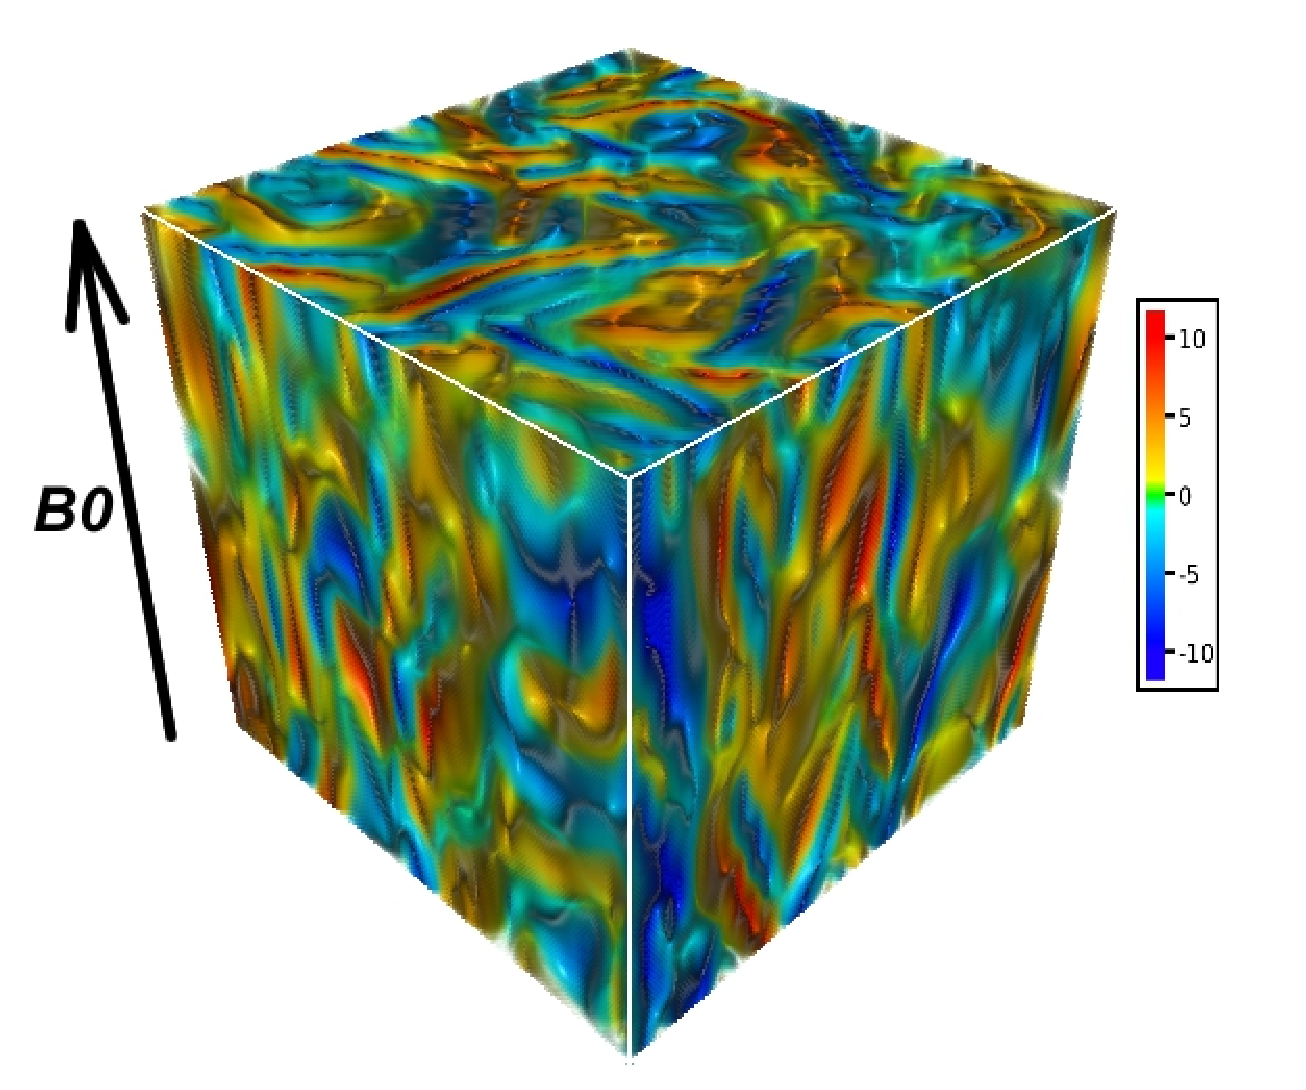
\includegraphics[width = 0.42\textwidth]{./Figures/Fig1_a}}
{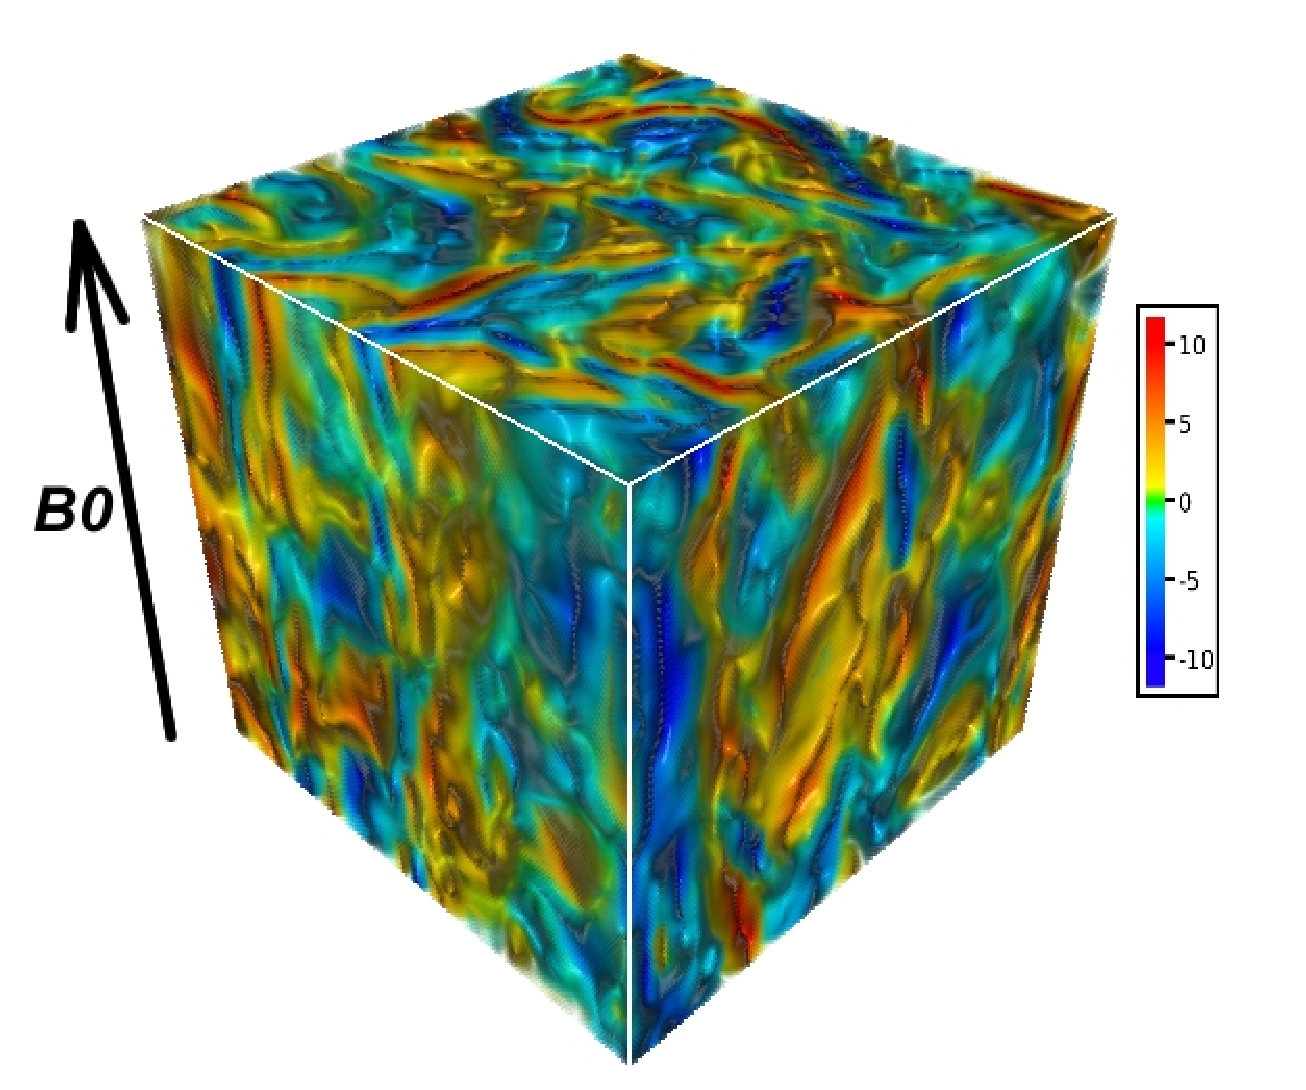
\includegraphics[width = 0.42\textwidth]{./Figures/Fig1_b}}
\caption{Three-dimensional view of the parallel current density $J_z(x,y,z)$. (Left) 
Incompressible and (Right) Compressible case with Mach number $M=0.25$ at $t/t_0 =2$.}
\end{center}
\end{figure*}

The MHD equations are solved numerically using 
a Fourier pseudospectral method with periodic 
boundary conditions in a cube of size  $L_{box}=2\pi L$; 
this scheme ensures exact energy conservation for the continuous time spatially discrete
equations\cite{ghost}. The discrete time integration is done with a high-order Runge-Kutta
method, and aresolution of ($256^3$) Fourier modes is considered. For the kinematic Reynolds
number $R=v_0L/\nu$ and the magnetic Reynolds number $R_m=v_0L/\eta$, 
we take $R=R_m= 1000$, which are limited here by available
spatial resolution. We consider a decaying simulation from an 
initial state with the kinetic 
and magnetic field fluctuations populating an annulus in Fourier k-space 
defined by a range of wavenumbers with
$ 3\leq k \leq4$, constant amplitudes, and random phases.

When the turbulence is fully-developed a broad range of 
scales develops, from the outer scale $L$ to 
the dissipation scale $l_d\approx L/32$. We then employ this
turbulent (fixed) MHD state in which to evolve the test
particles. The behavior of a test particle in an electromagnetic field 
is described by the nonrelativistic particle equation of motion:

\begin{equation}
  \frac{d\textbf{v}}{dt} = \alpha(\textbf{E} + \textbf{v} \times \textbf{B}), \ \ \ \  \frac{d\textbf{r}}{dt} = \textbf{v}.
\end{equation}
 
The nondimensional electric field \textbf{E} is obtained from Ohm's law 
normalized with $E_0= v_0 B_0/c$ as follows:

\begin{equation} about 
 \textbf{E} =  -\textbf{u}  \times \textbf{B} + \frac{\textbf{j}}{R_m}. 
\end{equation}

Finally the adimensional parameter $\alpha$ relates particles and MHD field parameters:
\begin{equation}
\alpha=Z\frac{m_p}{m}\frac{L}{\rho_{ii}},
\end{equation}
where $\rho_{ii}$ is the proton inertial length given 
by $\rho_{ii}=m_pc/(e\sqrt{4\pi\rho_0})$. The inverse $1/\alpha$ represents the noninal 
gyroradius, in units of $L$ and with velocity $v_0$ and measures the range of 
scales involved in the system (from the outer scale of turbulence to the particle
gyroradius). One could expect a value
$\alpha \gg 1$ specially for space physics and astrophysical plasmas.
This represent a huge computational challenge due to 
numerical limitations. As stated above, we consider here a dissipation length scale
$l_d=L/32$, which is also of the order of the current sheet thickness.



In the fixed MHD turbulence state, $10000$ test particles are 
randomly distributed 
in the computational box and the equation of motion of particles 
subject to the MHD
electromagnetic field are solved using a second-order Runge-Kutta method. 
Furthermore, we use high order spline interpolation to compute the field values on each
particle position.


Particles are initialized with Gaussian velocity distribution function with a 
root mean square (rms) value of the order of the Alfven velocity. It is well known that the 
particle gyroradius has a significant influence 
on acceleration, and our aim in this paper is to explore the compressibility effect on 
acceleration of large gyroradius 
and small gyroradius particles. 
In the next section we show two different compressible cases 
with Mach number $M=0.25$ and $M=0.1$, and an incompressible case. In all the cases the 
mean magnetic field is set to $B_0=10$. We present the behavior of protons with a 
nominal (speed $v_0$) gyroradius $1/32$, and electrons  ($m_e=m_p/1836$)
with nominal gyroradius $1/58752$.


\section{\label{sec:level3}RESULTS:}

In Figure 1 a three-dimensional view of the z-component of the current density $J_z(x,y,z)$ is shown at $t=2.5t_0$ for an incompressible case and a compressible case with $M=0.25$. It is observed that current sheets are aligned in the direction of the guide magnetic field. 
It can be seen that in both cases the structures are similar,
but more corrugated in the compressible case and smoother in the incompressible one. It is worth mentioning that we used the same 
initial conditions for all the simulations. Coherent structures like
these show the natural tendency of the MHD equations to develop strong gradients leading
to many reconection zones, which is well known to be one of the mechanisms behind
charged particle acceleration.

\begin{figure}[<h!>]
\begin{center}
\hspace*{0.4cm}{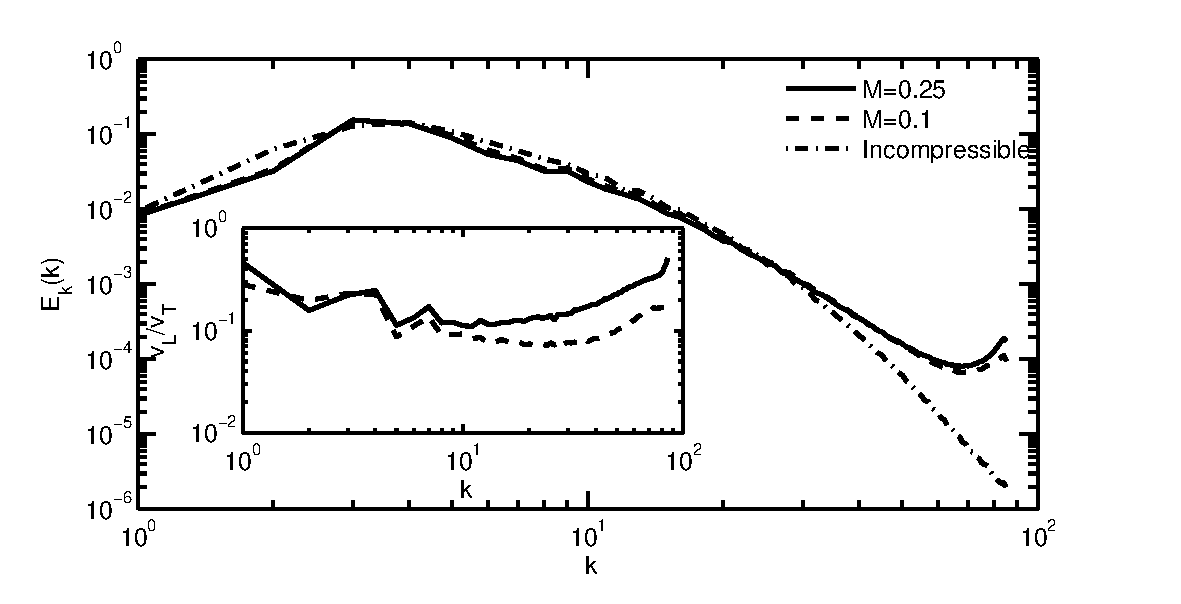
\includegraphics[width = 3.31in]{./Figures/Fig2_a}}\\
{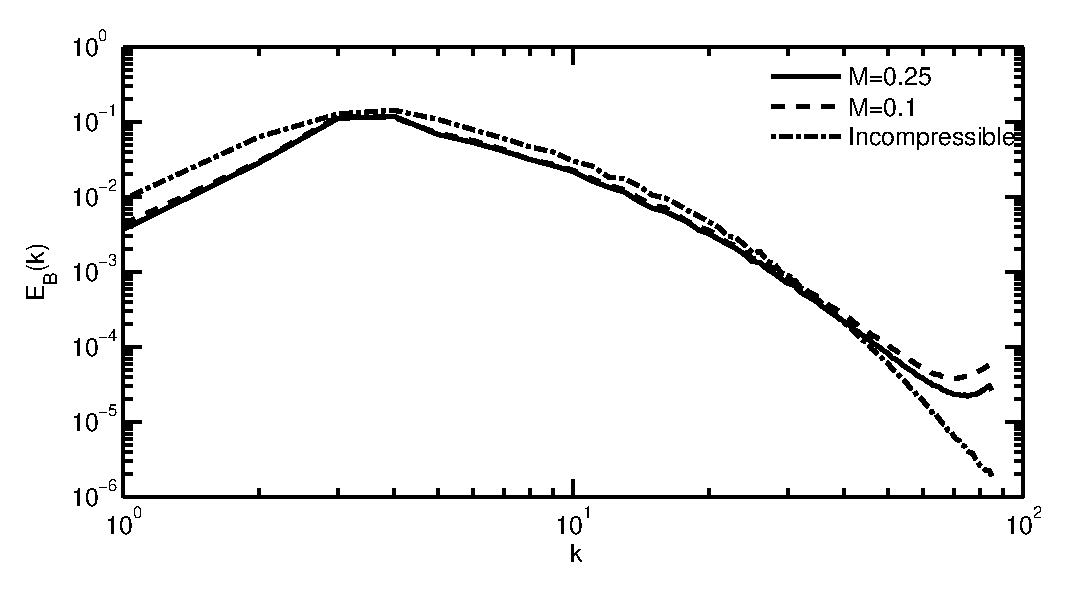
\includegraphics[width = 3.05in]{./Figures/Fig2_b}}\\
\caption{(Top) Kinetic energy spectrum for compressible cases with Mach 
numbers $M=0.25$ (solid line), $M=0.1$ (dashed line), and incompressible case 
(dashed-dot line); the inset shows the ratio between solenoidal
and irrotational (compressive) 
components of the velocity field for compressible runs. (Bottom) Magnetic energy spectrum
for the three cases mentioned before, using the same labels.}
\end{center}
\label{mean square velocity}
\end{figure}

Figure 2 shows the spectrum of kinetic (top) and magnetic energy (bottom) for the 
compressible cases with $M=0.25$ and $M=0.1$ cases, and the
incompressible case. In the inertial range there are almost no differences between the 
compressible and incompressible energy spectra for 
both magnetic and velocity fields, although slightly more energy at 
large scales is observed in the incompressible case. On the other hand, at wavenumbers beyond
the dissipation scale (that is, for $k\geq32$),  an excess of energy is observed as the Mach
number is increased. This feature is more evident for the kinetic energy spectrum
than for the magnetic energy spectrum. Since protons mostly interact with structures
of that size, this can be an important effect on proton acceleration.



In order to explore the importance of compressible effects on MHD fields,
we make a Helmholtz decomposition of the velocity field, presented
in the inset in Fig 2, where $v_T({\bf k}) = (\bf I - \hat k\hat k) u({\bf k)$ 
represents the solenoidal (incompressible) part 
and $v_L({\bf k}) = u({\bf{k}) - v_T({\bf k})$ is
the irrotational (compressive)
component. It is observed that at high $k$ the velocity field
spectrum is strongly compressive,
and that compression becomes more prominent at higher 
turbulent Mach number.

{\it Protons.}
Figure 3 shows the time evolution for the mean value of
the perpendicular $v_\perp = \sqrt{v_x^2+v_y^2}$ 
(top) and parallel $v_\parallel=v_z$ (bottom) proton velocity, 
relative to $B_0$, 
for the compressible ($M=0.25$, $M=0.1$) cases
and the incompressible case. 
The typical acceleration process observed in previous studies is
evident, proton are accelerated perpendicularly with respect to $B_0$, 
while they are less accelerated parallely. 

Moreover, the compressibiliy effect on particle acceleration 
is clearly observed.
Protons are highly accelerated as compressibility of the fluid increases 
for both perpendicular and parallel directions.
Acceleration of protons is also observed in the 
incompressible case (see inset plot) but
the value of the velocity reached at the end of the simulation is much lower than in both
compressible cases, even with relatively small values of the Mach number $M$ as the ones
considered here.

\begin{figure}[h!]
\begin{center}
{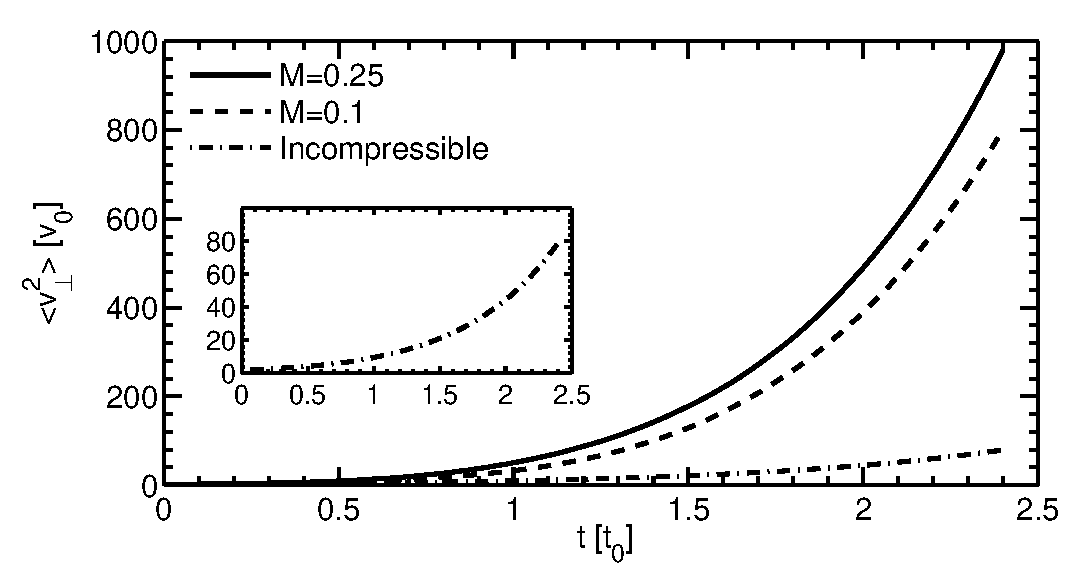
\includegraphics[width = 3.05in]{./Figures/Fig3_a}}
{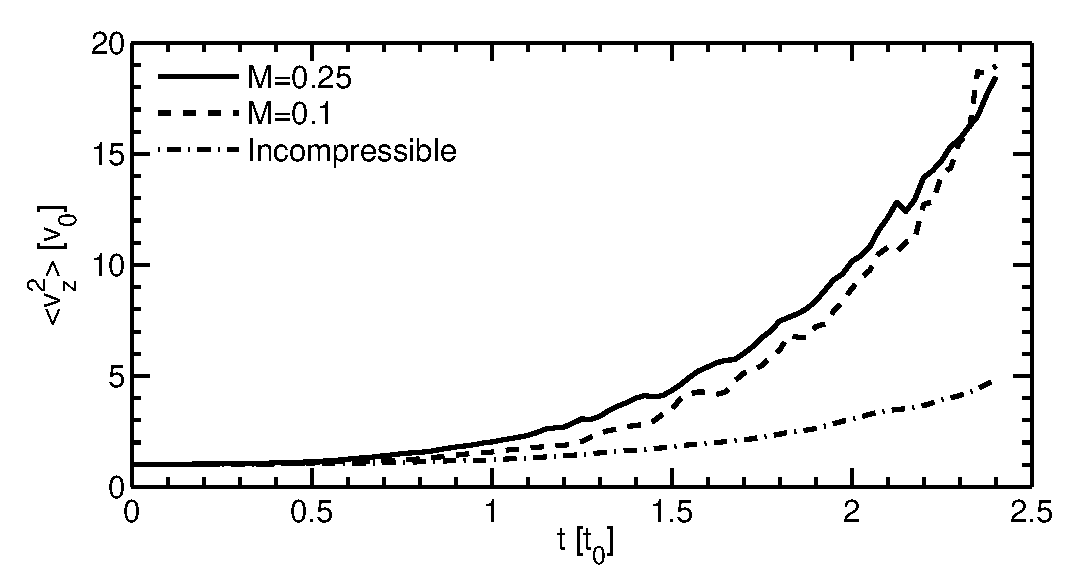
\includegraphics[width = 3.05in]{./Figures/Fig3_b}}
\caption{Particle mean square velocity as a function of time: (Top)
Proton perpendicular velocity $v_\perp = \sqrt{v_x^2 + v_y^2}$ 
for two different Mach number
cases, $M=0.25$ (solid line), $M=0.1$ (dashed line), and the
incompressible case (dash-dot line). 
(Bottom) Proton parallel velocity $v_\parallel=v_z$ for $M=0.25$, $M=0.1$, 
and incompressible case, with the
same labels for the lines.}
\end{center}
\label{mean square velocity}
\end{figure}

Figure 4 shows the probability distribution function (PDF) of the
perpendicular x-component (top) and of the parallel z-component (bottom) 
of the electric field 
for the compressible and incompressible cases. The PDF shows that, as compression increases,
long tails in the distribution arise and higher values of the perpendicular electric field 
are achieved. Additionally, the core part of the distribution function for the incompressible 
case is thicker than for the compressible cases. On the other hand, the PDF of the parallel electric field shows very 
little effect of increasing compressibility.

\begin{figure}
\begin{center}
{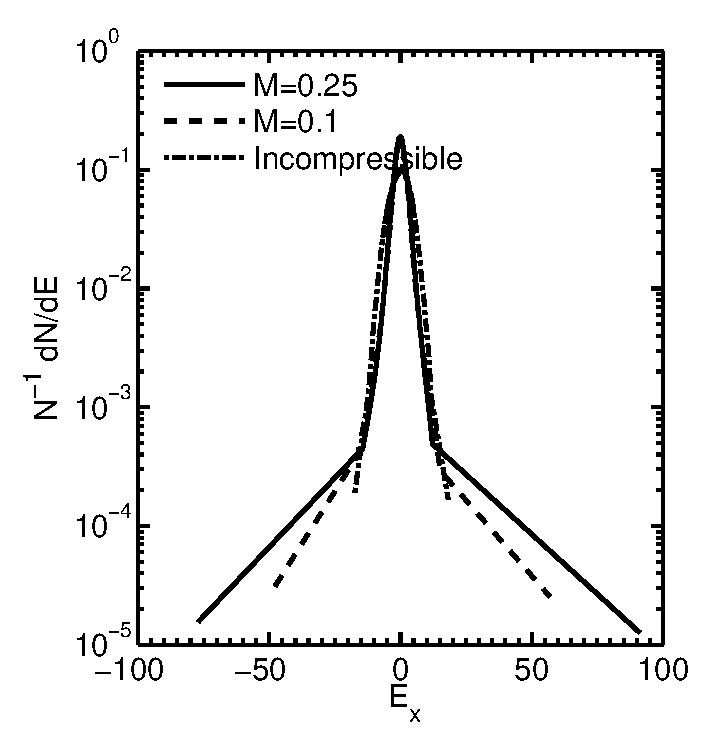
\includegraphics[width = 2.3in]{./Figures/Fig4_b}}
{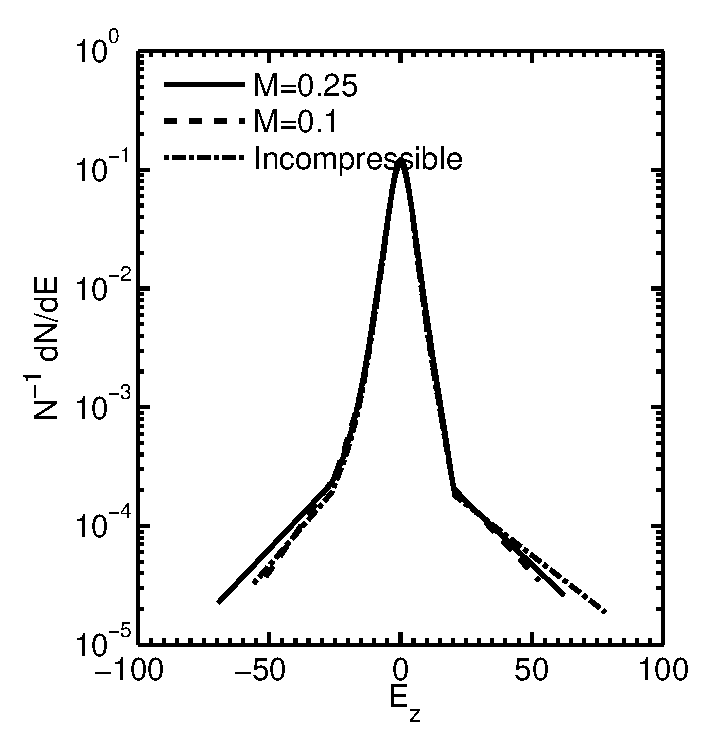
\includegraphics[width = 2.31in]{./Figures/Fig4_2}}
\caption{Probability density function of electric field components 
in the simulation. (Top) Perpendicular x-component 
for $M=0.25$ (solid line), $M=0.1$ (dashed line), and incompressible 
(dash-dot line). (Bottom) Parallel z-component of the electric field 
using the same labels.}
\end{center}
\label{mean square velocity}
\end{figure}


In order to better understand the dynamics of protons, in Figure
5 we show the current density $J_z(x,y,z)$ together
with the trajectory of one of the most energetic protons,
for the compressible $M=0.25$ case. The visualization was done using the software
VAPOR\cite{vapor}. It is observed that on the surrounding of the particle trajectory 
there are many current sheets, which contribute to the proton energization.

Figure 6 shows the values of quantities following the trajectory of the
most energetic proton, that is, the most energetic proton is identified
and the values of several quantities along the trajectory of this proton
are obtained: (a) the current density $J_z$, (b) electric field 
components $E_x, E_y, E_z$, (c) proton velocity components $v_x, v_y, v_z$ and (d) root
mean square displacement of the proton. The panels on the left correspond to the
compressible $M=0.25$ case, and the panels on the right correspond to the incompressible case.

%\vspace*{0.5cm}

\begin{figure}[h!]
\begin{center}
{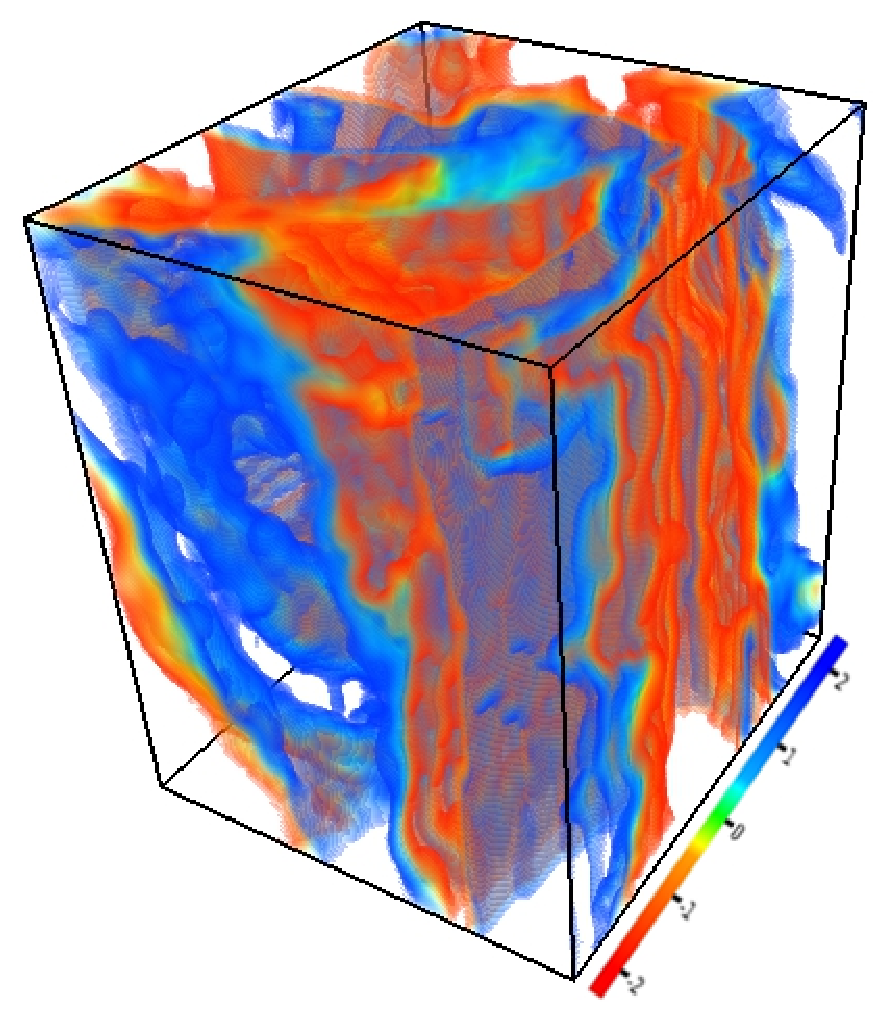
\includegraphics[width = 2.8in]{./Figures/Fig5_a}}
{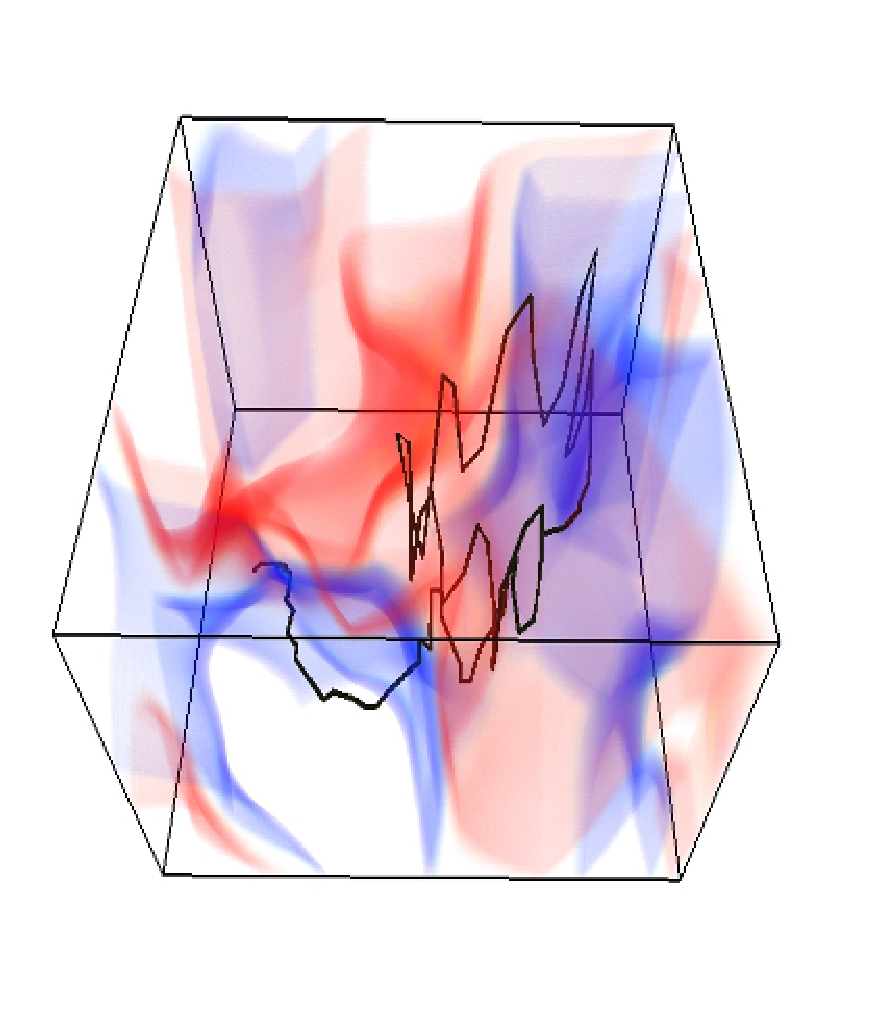
\includegraphics[height=2.8in, width = 3in]{./Figures/Fig5_b}}
\caption{(Top) View of the parallel current density $J_z(x,y,z)$.
(Bottom) Trajectory of one of the most energetic protons; the z-component of the current 
density is shown in the transparent volume rendering.}
\end{center}
\label{mean square velocity}
\end{figure}
It is observed that when there is a change of the sign in the 
current density $J_z$, there is also an increment in the 
perpendicular components of the electric field that 
the particle experience, and concurrently there is an increment 
of the proton velocity. This situation
is repeatedly observed in time as the energy of the proton increases.

A possible explanation for the change of sign in the current density is 
that the particle is entering and leaving two neighboring 
current sheets with different polarities while experiencing
a strong perpendicular electric field between those current sheets. 
The perpendicular electric field
is stronger as the compression of the fluid increases (this can be noticed
by comparing panels on the left and right of Figure 6).
Consequently the velocity increment is larger in the compressible case 
than in the incompressible case.
This situation can be 
generalized for many particles in the simulation, 
resulting in the increase of the root mean 
square velocity for the ensemble of particles. 

The reason for greater perpendicular electric field for the compressible cases 
can be understood in terms of the magnetic flux pileup that accompanies the 
interaction of adjacent flux tubes in turbulence\cite{ServidioEA10}. 
While current sheets typically form between interacting flux tubes, 
when the flux tubes are driven together by the turbulent flow, there
is also frequently a magnetic flux pileup near the boundary.
This compression of the magnetic field occurs in the incompressible case as well, 
but clearly can be greater when the material elements themselves are compressible.   
The pileup phenomenon is readily seen to be associated with 
reversal of the electric current density. Furthermore, the parallel magnetic flux increases
due to this compression, requiring a circulation of the perpendicular electric field vector, 
thus setting the scene for betatron acceleration \cite{Dalena2012}.

{\it Electrons.}
Figure 7 shows the time evolution for the perpendicular (top) 
and z-component (bottom) of electron
rms velocity for the compressible ($M=0.25$, $M=0.1$) and incompressible cases.

It should be mentioned that we are showing
a short time simulation of electrons here.
This is due to the high computational cost of integrating the trajectory of electrons
in a flow, as electrons require a small time step (to represent a physical 
small gyroradius).  The total time reached in the electron simulations
is of the order of almost 3000 
electron gyroperiods. 

Electrons present the typical parallel energization reported in previous works. 
Besides, there is no evidence that compression of the MHD fields enhance the electron 
acceleration and electrons gain almost the same energy regardless the compressible level of
the fluid.


\begin{figure*}[h!]
  \centering
  \begin{tabular}{@{}p{0.45\linewidth}@{\quad}p{0.45\linewidth}@{}}
    \subfigimg[width=\linewidth]{a)}{./Figures/Fig6_c_compress} &
    \subfigimg[width=\linewidth]{a)}{./Figures/Fig6_c_incompress} \\
    \subfigimg[width=\linewidth]{b)}{./Figures/Fig6_b_compress} &
    \subfigimg[width=\linewidth]{b)}{./Figures/Fig6_b_incompress} \\
    \subfigimg[width=\linewidth]{c)}{./Figures/Fig6_a_compress} &
    \subfigimg[width=\linewidth]{c)}{./Figures/Fig6_a_incompress} \\
    \subfigimg[width=\linewidth]{d)}{./Figures/Fig6_d_compress} &
    \subfigimg[width=\linewidth]{d)}{./Figures/Fig6_d_incompress}
  \end{tabular}
  \caption{(a) Parallel current density, (b) the three components of the electric field,
  (c) velocity components, and (d) rms displacement as function of time for the most
  energetic particle: (Left) compressible $M=0.25$ case and (Right) incompressible case. The
   gray vertical dashed-lines show the moments when current is reversed.}
\end{figure*}

\clearpage

Since the gyradius of electrons is smaller than any of the length
scales of structures in the fields, when electrons find a current sheet they travel 
along magnetic field lines and there is not so much difference between compressible and 
incompressible cases.

Also, the perpendicular rms velocity shows that electrons are initially accelerated 
but quickly exhibit a constant perpendicular energy. Constant 
perpendicular energy is consistent with near conservation of the 
magnetic moment, which is one of the adiabatic invariants of charged particle dynamics in
a magnetic field.

It is important to remark that over longer timescales, of the order 
of many turnover times, 
electrons can obtain very high parallel energy, and 
it is likely that the motion will 
no longer be adiabatic.  In that case, 
electrons can reach other regions and interact with 
structures that generate other possible acceleration mechanisms, 
such as those that involve 
pitch angle-scattering, betatron acceleration, etc.



\begin{figure}[<t>]
\begin{center}
{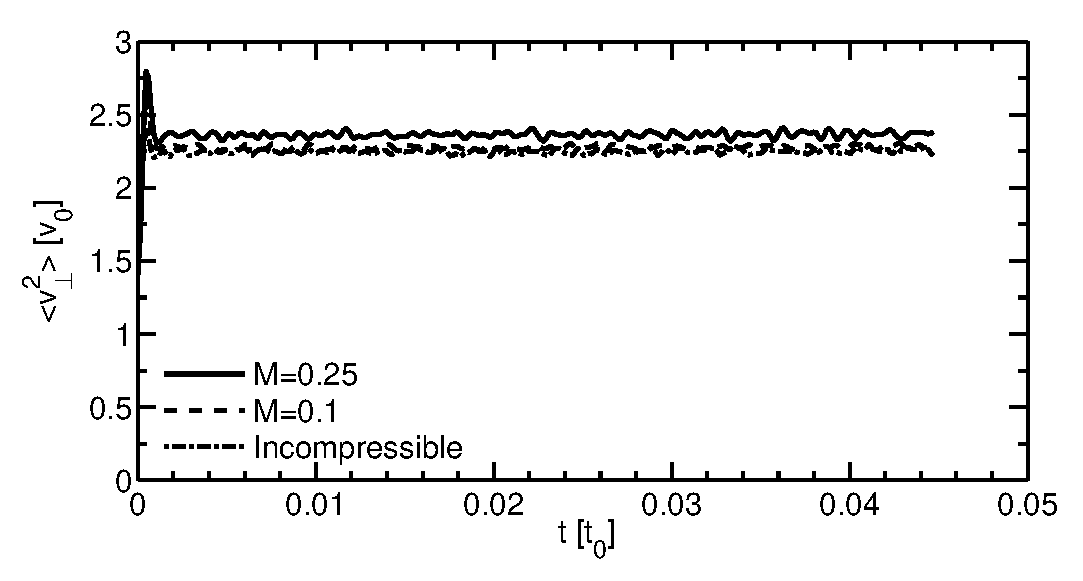
\includegraphics[width = 3.3in]{./Figures/Fig7_a}}
{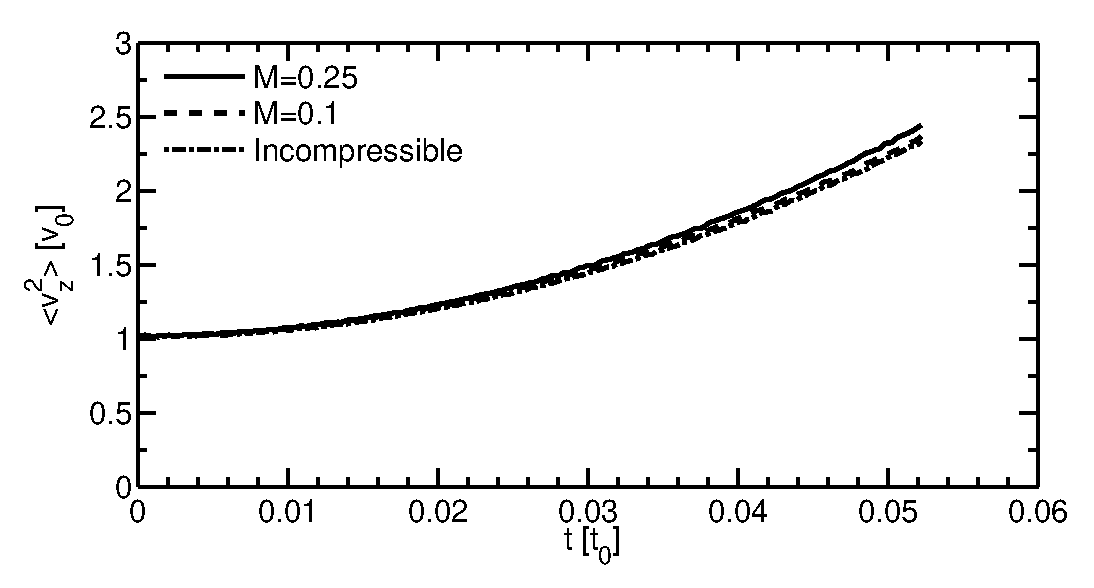
\includegraphics[width = 3.3in]{./Figures/Fig7_b}}
\caption{(Top) Time evolution of the perpendicular rms velocity for
electrons, for the compressible cases with $M=0.25$ (solid line), 
$M=0.1$ (dashed line), and the incompressible case (dot-dashed line). (Bottom) Time 
evolution of the parallel rms velocity for electrons, using the same notation.} 
\end{center}
\label{mean square velocity}
\end{figure}


\section{\label{sec:level4}DISCUSSION:}
We have investigated the effect of compressible MHD turbulence 
on particle energization, using test particle simulations in frozen electromagnetic fields
obtained from direct numerical solutions of the MHD equations. We found noticed that 
compression affects only the energization of large particle gyroradius (of the order of the 
dissipation length), and no effect of compression for small particle gyroradius is observed. 

Protons are accelerated by the perpendicular electric field generated on the interface of
current sheets, and they gain substantial energy as they encounter these structures. 
Moreover the perpendicular electric field between current sheets is greater as compression
of the fluid increases, leading to a higher proton acceleration. 

On the other hand, small gyroradii particles remain
magnetized and gain parallel energy as 
they travel along magnetic field lines almost aligned with $B_0$. No compression effect is
noted for these kind of particles and this is because the compressible modes in 
magnetohydrodynamics are perpendicular propagation modes ($k \perp B_0$), and as a result
no difference in the parallel electric field obtained from static MHD fields is presented.

In this paper we analyzed the case of weakly compressible turbulence, 
often appropriate to study the solar wind and other astrophysical scenarios, even though these plasmas
can sometimes attain a strongly compressible state 
($M \geq 1$). we can thus conclude that at least for low turbulent 
Mach number, compression can enhance particle energization associated 
with coherent structures and therefore it has important implications for the study of
particle acceleration by turbulent fields. In the incompressible case, which is the limit
of infinite sound wave velocity, protons can still be accelerated, but less than
in the compressible case. The incompressible case thus served as a reference to measure the
influence of compression on particle acceleration. Also, the incompressible case can 
represent a real physical scenario, like the fast solar wind which might energize particles as
well\cite{Bogdan2014}.

We close with a remark concerning the importance of trapping effects in acceleration of particles 
to higher energies in compressible turbulence. In general for effective energization the particles must be exposed to 
a suitable electric field, but also the trajectory of the particle must allow  
a long exposure time of the particle to the accelerating field. 

In the present case, parallel acceleration of electrons occurs when their gyroradii
are small compared to the width of mean field-aligned current channels, as noted previously by \citet{PD1}.
Analogous trapping effects due to confinement in magnetic ``islands'' has been noted in various systems from two dimensional  MHD
\cite{AmbrosianoEA88} to fully kinetic PIC simulations\cite{DrakeEA06}. In those scenarios small gyroradius particle are trapped
for a period of time sufficient for them to experience substantial parallel energization. Depending on parameters this may be 
either heating (more particles, lower energies) or acceleration (less particles but higher energy).
On the other hand, protons, having larger gyroradius, will not be easily trapped in current channels, 
which often are a few proton inertial scales in width. 

The perpendicular acceleration mechanism described previously \cite{PD1,Dalena2012} and elaborated on here, provides a way to accelerate protons (and heavier ions) due to pependicular electric fields.
The region of interaction between flux tubes provides the possibility of generating regions of effective
 acceleration that may lie between reversing currents. Although these may be very complex
 regions in three dimensions, in a simplified two dimensional picture, these can be flux
 pileup regions with gradients of the perpendicular electric field . This transversed
 compression of the  magnetic field may occur even when the turbulence is incompressible. However, it is 
 intuitively clear that compressibility
will permit greater pileup and greater perpendicular electric field gradients. In addition,
to produce an efficient accelerator, the particles must also be trapped in the accelerating 
region for sufficient time. The present numerical experiments 
also suggest that compressibility of the turbulence, acting near and within the regions 
between reversing 
currents, may provide substantially enhanced trapping for some particles. This is needed to 
explain the significantly greater perpendicular acceleration observed here when
the turbulence is compressible.  
\section*{Acknowldegments}
 
We acknowledge support from the following grants UBACyT 20020110200359, 20020100100315,
and PICT 2011-1529, 2011-1626, 2011-0454.

W.H. Matthaeus is partially supported by NASA LWS-TRT grant 
NNX15AB88G,Grand Challenge Research grant NNX14AI63G,
the Solar Probe Plus mission through the  Southwest Research Institute ISOIS 
project D99031L.
\vspace*{1cm}
\nocite{*}
\bibliographystyle{unsrtnat}
\bibliography{aipsamp}% Produces the bibliography via BibTeX.


\end{document}
%
% ****** End of file aipsamp.tex ******
